\documentclass[a4,danish]{article}
\documentclass[11pt,a4paper,twoside,openany,final]{memoir}
\usepackage[utf8]{inputenc}
\usepackage[twoside]{geometry}
%\usepackage[T1]{fontenc}
\usepackage[english]{babel}
\usepackage{amsmath}
\usepackage{amsfonts}
\usepackage{amsthm}
\usepackage[usenames,dvipsnames]{xcolor}
\usepackage{tikz}
\usepackage{amssymb}
\usepackage{graphicx}
\usepackage{flexisym}
\usepackage{hyperref}
\usepackage{xr}
\usepackage[all]{xy}
\usepackage{tikz-cd}
\usepackage{tkz-graph} % To make graphs
\usetikzlibrary{arrows}
\usepackage{tkz-tab}
\usepackage{hyperref}
\usepackage[style=authoryear,backend=bibtex,natbib]{biblatex}
\usepackage{filecontents}
\usepackage[english, status=draft]{fixme}
\fxusetheme{color}
\usepackage{cleveref} 
\usepackage[backgroundcolor=cyan]{todonotes}
\usepackage{wallpaper}
\usepackage{faktor}
\usepackage{nicefrac}
%\usepackage{txfonts}
\usepackage{afterpage} %Til at kunne indsætte tomme sider
\usepackage{pgfplots} %Til at kunne lave grafer
\usepackage{emptypage} %Fjerner sidetal og sidehoveder på tomme sider
\usepackage{multirow}
\usepackage{listings} % To use R language
\lstset{literate=%
{æ}{{\ae}}1
{å}{{\aa}}1
{ø}{{\o}}1
{Æ}{{\AE}}1
{Å}{{\AA}}1
{Ø}{{\O}}1
}
\lstset{ 
  language=R,                     % the language of the code
  basicstyle=\footnotesize\ttfamily, % the size of the fonts that are used for the code
  numberstyle=\tiny\color{blue},  % the style that is used for the line-numbers
  stepnumber=1,                   % the step between two line-numbers. If it is 1, each linewill be numbered
  numbersep=5pt,                  % how far the line-numbers are from the code
  backgroundcolor=\color{white},  % choose the background color. You must add \usepackage{color}
  showspaces=false,               % show spaces adding particular underscores
  showstringspaces=false,         % underline spaces within strings
  showtabs=false,                 % show tabs within strings adding particular underscores
%  frame=single,                   % adds a frame around the code
  rulecolor=\color{black},        % if not set, the frame-color may be changed on line-breaks within not-black text (e.g. commens (green here))
  tabsize=2,                      % sets default tabsize to 2 spaces
  captionpos=b,                   % sets the caption-position to bottom
  breaklines=true,                % sets automatic line breaking
  breakatwhitespace=false,        % sets if automatic breaks should only happen at whitespace
  keywordstyle=\color{RoyalBlue},      % keyword style
  commentstyle=\color{ForestGreen},   % comment style
  xleftmargin=0.5cm,
  xrightmargin=0.5cm
}


%\DisemulatePackage{setspace} START ALTERNATIV SPACING + MARGIN %
%\usepackage{setspace} %
%\doublespacing %
%\setlrmarginsandblock{5cm}{3cm}{*}
%\setulmarginsandblock{2.5cm}{2.5cm}{*}
%\checkandfixthelayout SLUT ALTERNATIV SPACING + MARGIN

\pgfplotsset{width=10cm,compat=1.9}

\begin{filecontents}{bibtest.bib}
@book{Clarke,
  title={Functional Analysis, Calculus of Variations and Optimal Control},
  author={Francis Clarke},
  volume={1},
  year={2013},
  publisher={Springer-Verlag London}
}
@book{Hansen,
  title={Measure Theory},
  author={Ernst Hansen},
  volume={4},
  year={2009},
  publisher={Department of Mathematical Sciences, University of Copenhagen}
}
@article{Topsoee,
  title={Compactness in spaces of measures},
  author={Flemming Topsøe},
  journal={Studia Mathematica},
  volume={36},
  number={3},
  year={1970},
  pages={195--212}
}
@book{Topsoee2,
  title={Topology and measure},
  author={Flemming Topsøe},
  volume={1},
  year={1970},
  publisher={Springer-Verlag, Berlin}
}
@article{Strassen,
  title={The existence of probability measures with given marginals},
  author={Strassen, Volker},
  journal={The Annals of Mathematical Statistics},
  volume={36},
  number={2},
  year={1965},
  pages={423--439}
}
@book{Hoffmann,
  title={Probability in Banach space},
  author={Jørgen Hoffmann-Jørgensen},
  volume={},
  year={1977},
  publisher={Springer}
}
@book{Rudin,
  title={Real and complex analysis},
  author={Walter Rudin},
  volume={3},
  year={1987},
  publisher={McGraw-Hill, Inc.}
}
@book{Rudin2,
  title={Functional analysis},
  author={Walter Rudin},
  volume={2},
  year={1991},
  publisher={McGraw-Hill, Inc.}
}
@book{Aliprantis,
  title={Infinite Dimensional Analysis: A Hitchhiker's Guide},
  author={Charalambos D. Aliprantis and Kim C. Border},
  volume={3},
  year={2006},
  publisher={Springer-Verlag Berlin}
}
@article{Lindvall,
  title={On Strassen's Theorem on stochastic domination},
  author={Torgny Lindvall},
  journal={Electronic Communications in Probability},
  volume={4},
  number={7},
  year={1999},
  pages={51--59}
}
@book{Billingsley,
  title={Convergence of Probability Measures},
  author={Patrick Billingsley},
  volume={2},
  year={2013},
  publisher={John Wiley and Sons}
}
@article{Kamae,
  title={Stochastic inequalities on partially ordered spaces},
  author={Teturo Kamae and Ulrich Krengel and George L. O'Brien},
  journal={The Annals of Probability},
  volume={5},
  number={6},
  year={1977},
  pages={899--912}
}
@book{Sokol,
  title={Advanced Probability},
  author={Alexander Sokol and Anders Rønn-Nielsen},
  volume={4},
  year={2016},
  publisher={Department of Mathematical Sciences, University of Copenhagen}
}
@book{Bladt,
  title={Matrix–exponential distributions in Applied Probability},
  author={Mogens Bladt and Bo Friis Nielsen},
  volume={1},
  year={2017},
  publisher={Springer (Pending)}
}
@article{Rosenblum,
  title={Simple Examples of Estimating Causal Effects Using Targeted Maximum Likelihood Estimation},
  author={Michael Rosenblum and Mark J. van der Laan},
  journal={U.C. Berkeley Division of Biostatistics Working Paper Series},
  volume={Working Paper 262},
  year={2010}
}
@Inbook{Kennedy,
author="Kennedy, Edward H.",
editor="He, Hua
and Wu, Pan
and Chen, Ding-Geng (Din)",
title="Semiparametric Theory and Empirical Processes in Causal Inference",
bookTitle="Statistical Causal Inferences and Their Applications in Public Health Research",
year="2016",
publisher="Springer International Publishing",
address="Cham",
pages="141--167",
isbn="978-3-319-41259-7",
doi="10.1007/978-3-319-41259-7_8",
url="https://doi.org/10.1007/978-3-319-41259-7_8"
}
@book{TargetedLearning,
  title={Targeted Learning in Data Science},
  author={Mark J. van der Laan and Sherri Rose},
  volume={1},
  year={2011},
  publisher={Springer}
}
@article{Wikkelsoee,
  title={Prediction of postpartum blood transfusion -- risk factors and recurrence.},
  author={AJ Wikkelsøe and S Hjortøe and TA Gerds and AM Møller and J Langhoff-Roos}, 
  journal={The journal of maternal-fetal and neonatal medicine},
  volume={27},
  number={16},
  year={2014}
}
@book{Causality,
  title={Elements of causal inference},
  author={Jonas Peters and Dominik Janzing and Bernhard Schölkopf},
  volume={1},
  year={2017},
  publisher={MIT Press}
}
@book{Asymptotic,
  title={Asymptotic Statistics},
  author={A. W. Van der Vaart},
  volume={3},
  year={2000},
  publisher={Cambridge University Press}
}
@article{PPHcause,
  title={Recent Advances in the Management of Major Postpartum Haemorrhage - A Review},
  author={P Reddi Rani1 and Jasmina Begum}, 
  journal={Journal of Clinical and Diagnostic Research},
  volume={11},
  number={2},
  year={2017}
}
@Manual{SuperLearner,
    title = {SuperLearner: Super Learner Prediction},
    author = {Eric Polley and Erin LeDell and Chris Kennedy and Mark {van der Laan}},
    year = {2018},
    note = {R package version 2.0-23},
    url = {https://CRAN.R-project.org/package=SuperLearner}
}
@Article{tmle,
    title = {{tmle}: An {R} Package for  Targeted Maximum Likelihood Estimation},
    author = {Susan Gruber and Mark J. {van der Laan}},
    journal = {Journal of Statistical Software},
    year = {2012},
    volume = {51},
    number = {13},
    pages = {1--35},
    url = {http://www.jstatsoft.org/v51/i13/},
}



\end{filecontents}

\addbibresource{bibtest.bib}


\chapterstyle{verville}


\setlength{\parindent}{0em}
\setlength{\parskip}{1em}
\renewcommand{\baselinestretch}{1}


\DeclareMathOperator{\supp}{supp}
\DeclareMathOperator{\Ext}{Ext}
\DeclareMathOperator{\Aut}{Aut}
\DeclareMathOperator{\Ran}{Ran}
\DeclareMathOperator{\Prob}{Prob}
\DeclareMathOperator{\conv}{conv}
\DeclareMathOperator{\AR}{AR}
\DeclareMathOperator{\Homeo}{Homeo}

\makepagestyle{abs}
    \makeevenhead{abs}{}{}{}
    \makeoddhead{abs}{}{}{}
    \makeevenfoot{abs}{}{\scshape I }{}
    \makeoddfoot{abs}{}{\scshape  I }{}
    %\makeheadrule{abs}{\textwidth}{\normalrulethickness}
    %\makefootrule{abs}{\textwidth}{\normalrulethickness}{\footruleskip}
\pagestyle{abs}


\makepagestyle{cont}
    \makeevenhead{cont}{}{}{}
    \makeoddhead{cont}{}{}{}
    \makeevenfoot{cont}{}{\scshape II }{}
    \makeoddfoot{cont}{}{\scshape  II }{}
    %\makeheadrule{abs}{\textwidth}{\normalrulethickness}
    %\makefootrule{abs}{\textwidth}{\normalrulethickness}{\footruleskip}
\pagestyle{cont}

\newcommand{\lv}{\lVert}
\newcommand{\rv}{\rVert}


\renewcommand\chaptermarksn[1]{}
\nouppercaseheads
\createmark{chapter}{left}{shownumber}{}{.\space}
\makepagestyle{dut}
    \makeevenhead{dut}{\scshape\rightmark}{}{}
    \makeoddhead{dut}{\scshape\leftmark}{}{}
    \makeevenfoot{dut}{}{\scshape $-$ \thepage\ $-$}{}
    \makeoddfoot{dut}{}{\scshape $-$ \thepage\ $-$}{}
    \makeheadrule{dut}{\textwidth}{\normalrulethickness}
    \makefootrule{dut}{\textwidth}{\normalrulethickness}{\footruleskip}
\pagestyle{dut}

\makepagestyle{chap}
    \makeevenhead{chap}{}{}{}
    \makeoddhead{chap}{}{}{}
    \makeevenfoot{chap}{}{\scshape $-$ \thepage\ $-$}{}
    \makeoddfoot{chap}{}{\scshape $-$ \thepage\ $-$}{}
    \makefootrule{chap}{\textwidth}{\normalrulethickness}{\footruleskip}
\copypagestyle{plain}{chap}

\newcommand{\R}{\mathbb{R}}
\newcommand{\C}{\mathbb{C}}
\newcommand{\N}{\mathbb{N}}
\newcommand{\E}{\mathrm{E}}
\newcommand{\Var}{\mathrm{Var}}
\newcommand{\mbr}{(X,\mathcal{A})}
\newcommand{\Z}{\mathbb{Z}}
\newcommand{\Q}{\mathbb{Q}}
\newcommand{\F}{\mathcal{F}}
\newcommand{\A}{\mathcal{A}}
\newcommand{\cc}{C_c}
\newcommand{\PP}{\mathcal{P}}
\newcommand{\B}{\mathcal{B}}
\newcommand{\ee}{\epsilon}
\newcommand{\la}{\lambda}
\renewcommand{\H}{\mathcal{H}}
\newcommand{\pp}{\text{Prob}}
\newcommand{\U}{\mathcal{U}}
\newcommand{\dd}{\mathrm{d}}

\newcommand{\nocontentsline}[3]{}
\newcommand{\tocless}[2]{\bgroup\let\addcontentsline=\nocontentsline#1{#2}\egroup} % Fjern sections fra Table of Contents

\makeatletter
\newcommand{\Spvek}[2][r]{%
  \gdef\@VORNE{1}
  \left(\hskip-\arraycolsep%
    \begin{array}{#1}\vekSp@lten{#2}\end{array}%
  \hskip-\arraycolsep\right)}

\def\vekSp@lten#1{\xvekSp@lten#1;vekL@stLine;}
\def\vekL@stLine{vekL@stLine}
\def\xvekSp@lten#1;{\def\temp{#1}%
  \ifx\temp\vekL@stLine
  \else
    \ifnum\@VORNE=1\gdef\@VORNE{0}
    \else\@arraycr\fi%
    #1%
    \expandafter\xvekSp@lten
  \fi}
\makeatother

\def\acts{\curvearrowright}

\newcommand{\K}{\mathbb{K}}

\newtheoremstyle{break}
	{\topsep}{\topsep}
	{\bfseries}{}
	{\newline}{}
\theoremstyle{break}
\newtheorem{theorem}[subsection]{Theorem}
\newtheorem{lemma}[subsection]{Lemma}
\newtheorem{proposition}[subsection]{Proposition}
\newtheorem{corollary}[subsection]{Corollary}
\newtheorem{definition}[subsection]{Definition}
\newtheoremstyle{Break}
	{\topsep}{\topsep}
	{}{}
	{\bfseries}{}
	{\newline}{}
\theoremstyle{Break}
\newtheorem{example}[subsection]{Example}
\newtheorem{remark}[subsection]{Remark}
\newtheorem{note}[subsection]{Note}
\setcounter{secnumdepth}{0}
\usepackage{xpatch}
\xpatchcmd{\proof}{\ignorespaces}{\mbox{}\\\ignorespaces}{}{}

\newcommand*{\diff}{\mathop{}\!\mathrm{d}}

\newcommand\blankpage{%
    \null
    \thispagestyle{empty}%
    \addtocounter{page}{-1}%
    \newpage}
    
\DeclareNameAlias{sortname}{last-first} % Med flere forfattere bliver alle navne på formen
\DeclareNameAlias{default}{last-first} % : "LastName, FirstName MiddleName

\newcommand{\blank}{\makebox[1ex]{\textbf{$\cdot$}}} % Command to placeholder

\newcommand{\indep}{\rotatebox[origin=c]{90}{$\models$}} % Independent symbol

\title{Statistical analysis of shapes}
\author{Mads and Anders}
\date{\today}

%%% Local Variables:
%%% mode: latex
%%% TeX-master: "mainfile"
%%% End:


\begin{document}
\maketitle
\newpage


\begin{abstract}
\noindent
Performing statistics on data consisting of shapes rather than numerical values requires geometric constructions on the manifold of shapes. In this project we develop concepts of Riemannian geometry which are used to define the variance and mean of a random variable with values in a finite-dimensional manifold. We construct the infinite-dimensional manifolds of parametrized and un-parametrized smooth curves in $\R^2$ called shape spaces. We equip the shape spaces with different metrics some of which can be used to determine the distance between two shapes. Finally we discuss if the theory of statistics on finite-dimensional manifolds can be generalized to the infinite-dimensional shape spaces.

\end{abstract}
\newpage
\tableofcontents
\newpage


\section*{Introduction}
\label{sec:introduction}

A continuously evolving part of statistics is the area of statistical shape analysis where data consists of geometrical shapes instead of observations with a clear numerical representation. In order to perform statistics on geometric shapes, concepts such as distance between shapes has to be well-defined and one has to construct measures on a suitable shape space.

In this project we begin with an introduction of some concepts from Riemannian geometry which are crucial when trying to define statistics on a shape space. This introduction assumes some knowledge of the basic construction of Riemannian manifolds and sets out to define geodesics and the curvature of a manifold $M$ through an abstract construction using the Levi-Civita connection.

The next section introduces generalizations of variance and mean of a $M$-valued random variable when $M$ is a finite-dimensional Riemannian manifold. The mean is generalized through the concept of Riemannian centers of mass and several results are presented regarding the existence and uniqueness of such centers of mass. These results are based on considerations on the curvature of the manifold and the explicit expressions of Riemannian centers of mass are related to the inverse of the exponential map defined through geodesics in the previous section.

Next we introduce the manifolds of parametrized and unparametrized smooth curves in $\R^2$, Imm$(S^1, \R^2)$ and $\mathcal{I}$ respectively. We consider geometric shapes as elements of the latter, and we define metrics on both manifolds. Using these metrics we define the length of a path in the shape space, which can be seen as a deformation of one shape into another. The distance between two shapes is then defined to be the infimum of the length of all paths between the two. We show that a simple metric imposed on $\mathcal{I}$, the $L^2$-metric, induces a vanishing distance function such that the distance between two shapes can be made arbitrarily small.

Since the $L^2$-metric vanishes on $\mathcal{I}$ we turn towards almost local metrics as a way of imposing suitable metrics on $\mathcal{I}$. Almost local metrics are defined and we show that a certain almost local metric separates points in $\mathcal{I}$. The geodesic equations of $\mathcal{I}$ equipped with an almost local metric are not necessarily well-defined, but an example is given of when the length of a path between two shapes can explicitly be computed.

The last section consists of a discussion on the issues of defining statistical concepts on the shape space. Even if the almost local metrics induce a point-separating distance function on $\mathcal{I}$, there are still challenges with generalizing the constructions from the finite-dimensional case. We reflect upon these challenges and try to point towards further work needed to be done to solve these challenges.

\newpage
\section*{Concepts of Riemannian geometry}
\label{sec:concepts_of_Riemannian_geometry}

\subsection{Notation}

In the following $M$ denotes a smooth manifold and $TM$ is the tangent bundle of $M$ and $\mathcal{T}(M)$ denotes the space of all vector fields on $M$. For $I \subset \R$, $\gamma: \; I \rightarrow M$ is a curve in $M$, i.e. a smooth map.  

\subsection{Connections}

To consider the geodesic distance between two points in a manifold, geodesics need to be defined in a coordinate-invariant way such that the distance is independent of the coordinate charts. One property of geodesics in a Euclidean space, straight lines, is that they have acceleration $0$. In order to make sense of acceleration of a curve in a manifold, we need to be able to compute "differences" between tangent spaces along the curve. \textit{Connections} are exactly a way of making computations between tangent spaces possible - they allow us to differentiate vector fields along curves.\\[0.2 cm]
Since our use of connections is to define geodesics, we define connections in the tangent bundle of a manifold (instead of defining them generally on smooth sections of vector bundles) follwing chapter $4$ of \hl{RiemannLee}. 

\begin{definition}
A connection in $TM$ is a map
\begin{align*}
\nabla \, : \, \mathcal{T}(M) \times \mathcal{T}(M) \rightarrow \mathcal{T}(M),
\end{align*}
written $(X, Y) \mapsto \nabla_X Y$ satisfying (for $f$, $g \in C^\infty(M)$ and $a$, $b \in \R$);
\begin{align*}
& a) \; \nabla_{fX_1 + gX_2} Y = f\nabla_{X_1} Y + g\nabla_{X_2} Y \; \; \; \; & \text{(linearity over} \; C^\infty(M) \, \text{in} \, X) \\
& b) \; \nabla_X (aY_1 + bY_2) = a\nabla_X Y_1 + b\nabla_X Y_2 & \text{(linearity over} \; \R \, \text{in} \, Y) \\
& c) \; \nabla_X (fY) = f\nabla_X Y + (Xf)Y & \text{(product rule)}
\end{align*}
\end{definition}

In accordance with connections allowing "differences" between tangent spaces, $ \nabla_X Y $ is called the $\textit{covariant derivative of Y in the direction of X}$. Note that the product rule for connections is identical to the product rule of derivations. To use connections to derivate along curves, we need the definition of a \textit{vector field along a curve}, which is a smooth map $V: \, I \rightarrow TM$ such that $V(t) \in T_{\gamma(t} M$ for all $t \in I$. The prime example of a vector field along a curve is its velocity, $\dot{\gamma}(t) \in T_{\gamma(t} M$, which acts on functions, $f \in C^\infty(M)$, by
\begin{align*}
\dot{\gamma}(t) f = \frac{\text{d}}{\text{dt}} (f \circ \gamma)(t).
\end{align*} 
We denote by $\mathcal{T}(\gamma)$ all vector fields along $\gamma$. 
To define geodesics all we now need is to define what is means to take the covariant derivative of $V \in \mathcal{T}(\gamma)$ along $\gamma$. This covariant derivative is noted $D_t V$ and is has the following properties.

\begin{lemma}
Let $\nabla$ be a linear connection on $M$. For each $\gamma: \; I \rightarrow M$, $\nabla$ determines a unique operator
\begin{align*}
D_t: \; \mathcal{T}(\gamma) \rightarrow \mathcal{T}(\gamma),
\end{align*} 
satisfying (for $f$, $g \in C^\infty(I)$ and $a$, $b \in \R$);
\begin{align*}
& a) \; D_t(aV + bW) = aD_tV + bD_tW \; \; \; \; & \text{(linearity over} \; \R \\
& b) \; D_t(fV) = \dot{f}V + fD_tV & \text{(product rule)} \\
& c) \; \text{If V is extendible, then for any extension} \, \tilde{V} \, \text{of V}, \; \; D_tV(t) = \nabla_{\dot{\gamma}(t)} \tilde{V}.
\end{align*}
\end{lemma}
\begin{proof}
Proof of Lemma 4.9 in \hl{RiemannLee}
\end{proof}

$V$ is said to be extendible if it can be constructed by any vector field on $M$, $\tilde{V}$ by letting $V(t) := \tilde{V}_{\gamma(t)}$. This is not always the case; if $V$ is the velocity of an intersecting curve $\gamma$ with different covariant derivative at the intersection times. The covariant derivative of the velocity of a curve is now used to define a geodesic.

\begin{definition}
Let $\nabla$ be a linear connection on $M$ and $\gamma$ a curve in $M$. The acceleration of $\gamma$ is $D_t \dot{\gamma}(t)$. If this vector field is zero, $D_t \dot{\gamma}(t) \equiv 0$, then $\gamma(t)$ is a geodesic with respect to $\nabla$
\end{definition}

It follows from Theorem $4.10$ in \hl{RiemannLee} that for any manifold, $M$, with a linear connection, for any $p \in M$ and $V \in T_pM$ and $t_0 \in \R$ there exists an un-extendable geodesic, $\gamma_V: \; I \rightarrow M$, with $\gamma(0) = p$ and $\dot{\gamma}(0) = V$. The geodseic is called the (maximal) geodesic with initial value $p$ and initial velocity $V$. \\[0.2 cm]

In this construction of geodesics the only necessary structure of $M$ is that it should be a smooth manifold. When $M$ is also equipped with a Riemannian metric, making $M$ a Riemannian manifold, the choice of connection (determining the geodesics) should in some way respect the metric. Geodesics resulting from this specific choice of connection are called \textit{Riemannian geodesics}.

\subsection{Riemannian Geodesics and the Exponential Map}

Let $M$ be Riemannian manifold with metric $g$. To define Riemannian geodesics, we must first choose a specific connection on $M$ with two properties - \textit{compatability w.r.t. $g$} and \textit{symmetric} (these properties arise when trying to generalize the tangential conenction of a manifold submersed in $\R^n$).

\begin{definition}
A conneciton on $M$ is \textit{compatible with g} if the product rule
\begin{align*}
\nabla_X (Y, Z) = \langle \nabla_X Y, Z \rangle + \langle Y, \nabla_X Z \rangle
\end{align*}
holds for all vector fields, $X, Y$ and $Z$.
\end{definition}

By Lemma $5.2$ in \hl{RiemannLee} this condiiton is equivalnt with
\begin{align*}
\frac{d}{dt} \langle V, W \rangle = \langle D_t V, W \rangle + \langle V, D_t W \rangle,
\end{align*} 
for $V, W$ being vector fields along any curve $\gamma$. \\[0.2 cm]

The defintion of a symmetric connection involves the Lie bracket of two vector fields. If we think of vector fields on $M$, $X, Y$, as derivtations acting on $C^\infty (M)$, then the Lie brakcet of $X$ and $Y$, $[X , Y]$, is the vector field (derivation) which acts on $f \in C^\infty (M)$ by

\begin{align*}
[X , Y] (f) := X(Y(f)) - Y(X(f)),
\end{align*}
where $X(f) \in C^\infty (M)$ is the function which evaluated at $p$ is the derivative of $f$ at $p$ in the direction of $X(p)$. 

\begin{definition}
A connection on $M$ is \textit{symmetric} if 
\begin{align*}
\nabla_X Y - \nabla_Y X \equiv [X, Y].
\end{align*}
\end{definition}

(Note that interchanging $X$ and $Y$ makes sense, since $[X, Y] = - [Y, X]$.) A symmetric connection is also called \textit{torsion free}, which corresponds to the vector fields along any curve not being "twisted" when they are parallel transported along the curve. By the Fundamental Theorem of Riemannian Geometry, given any Riemannian manifold $(M,g)$, there exists a unique connection, $\nabla$, on $M$ that is symmetric and compatible with $M$. This connection is called the Riemannian connection of the Levi-Civita connection, and geodesics with respect to this connection are called Riemannian geodesics. Since this choice of connection is unique, geodesics in a Riemannian manifold will always mean Riemannian geodesics. Such geodesics can be used to define the exponential map, $\exp: \; TM \rightarrow M$.  

\begin{definition}
Given a point $p$ in a Riemannian manifold, $M$, and a vector $v \in T_p M$, the \textit{exponential map} is defined by $\exp_p (v) = \gamma_v(1)$ where $\gamma$ is the unique geodesic with $\gamma(0) = p$ and $\dot{\gamma}(0) = v$.
\end{definition}

The exponential map pushes a point $p \in M$ a unit distance in the direction of $v$ along the geodesic $\gamma$. Since $\dot{\gamma}(0) = v$, the differential of $\exp_p$ at $p$ is $v$, and so $\exp_p$ is a local diffeomorphism by the implicit function theorem. A Riemannian manifold is said to be \textit{geodesically complete} if every un-exentedable geodesic is defined on all of $\R$, and it follows from the Hopf-Rinow theorem that a manifold is geodesically complete if and only if, there exists a $p \in M$ such that $\exp$ is defined on all of $T_p M$.\\[0.2 cm] 
If the geodesic $\gamma_v$ is defined on all of $\R$, one can investigate for which values of $t$, the extended geodesic, $\gamma_v(t) = \exp_p (t v)$ is still a geodesic from $p$ to $\exp_p (t v)$. If $\gamma_v$ is a geodesic up to time $t_0$ and not after $t_0$, then $t_0$ is called a \textit{cut point}. The set of all cut points of all geodesics starting at $p$ is called the \textit{cut locus} and is denoted $C(p)$.

\subsection{Curvature}

When defining statistical propoerties such as mean and variance on Riemannian manifolds, measuring geometric propoerties of the manifold is needed. It is therefore of interest to determine on which manifolds these measurements are identical - that is to determine which manifolds are (locally) isomorphic. One way of determining this is to find a local invariant property of a manifold which is preserved by isometries (such that measurements of length are preserved). This property will be the \textit{curvature}. \\[0.2 cm]

Let $M = \R^n$ equipped with the Euclidean metric and consider a vector field $Z$. Given two other vector fields, $X$ and $Y$, we can now differentiate $Z$ first along $X$ and then along $Y$ by using the Riemannian connection;
\begin{align*}
\nabla_Y \nabla_X Z,
\end{align*}
and in the opposite order by $\nabla_X \nabla_Y Z$. If $R^n = R^2$ and $X$ and $Y$ where just vector fields corresponding to local coordinates then, by commutativity of second order derivatives,
\begin{align*}
\nabla_Y \nabla_X Z - \nabla_X \nabla_Y Z = \nabla_Y (\partial_1 Z^k \partial_k) - \nabla_X (\partial_2 Z^k \partial_k) = \partial_2 \partial_1 Z^k \partial_k - \partial_1 \partial_2 Z^k \partial_k = 0.
\end{align*}
But if $X$ and $Y$ are arbitrary vector fields, this identity does not necessarily hold, since
\begin{align*}
\nabla_Y \nabla_X Z - \nabla_X \nabla_Y Z = XYZ^k \partial_k - YXZ^k \partial_k = (XYZ^k - YXZ^k)\partial_k,
\end{align*}
where $XYZ^k = X \left( Z \left( Z^k \right) \right)$ to ease notation. The action of the Lie bracket of $X$ and $Y$ is recognized in the parenthesis, and thus for $\R^n$ the following identity holds;
\begin{align}\label{flat}
\nabla_Y \nabla_X Z - \nabla_X \nabla_Y Z = \nabla_{[X,Y]} Z.
\end{align}
Since this identity depends on the Levi-Civita connection, it holds for all manifolds isometric to $\R^n$, and manifolds for which \ref{flat} holds will be called \textit{flat} manifolds. To define the curvature of a manifold is then to determine how "un-flat" the manifold is, by considering the \textit{curvature transformation}, $R: \; \mathcal{T}(M) \times \mathcal{T}(M) \times \mathcal{T}(M) \rightarrow \mathcal{T}(M)$, defined by
\begin{align*}
R(X,Y)Z =  \nabla_Y \nabla_X Z - \nabla_X \nabla_Y Z - \nabla_{[X,Y]} Z,
\end{align*}
which is identically zero for flat manifolds. The curvature transformation can then be used to determine the curvature of a vector field by defining the \textit{curvature tensor};

\begin{definition}
The curvature on a Riemannian manifold is
\begin{align*}
Rm(X,Y,Z,W) = \langle R(X,Y)Z, W \rangle,
\end{align*}
with $\langle \cdot ,  \cdot \rangle $ being the inner product determined by the Riemannian metric.
\end{definition}



\section{Mean and variance}
\label{sec:mean_and_variance}

In order to perform statistics on shapes we must first try to define central statistical concepts on manifolds. In this section we focus on a geodsically complete Riemannian manifold, $(M, g)$, of dimension $n$, and present ways of defining the mean, variance and covariance of $M$-valued random variables. Given an underlying probability space, $(\Omega, \mathcal{F}, P)$, an $M$-valued random variable is a $\mathcal{F}/\mathcal{B}(M)$ measurable map, $X: \, \Omega \rightarrow M$, and we denote by $x = X(\omega)$ a realization of $X$ on $M$.\\[0.2 cm]
In order to perform statistics on $M$ we need to construct a measure on $M$. This measure is induced by the metric $g$ in the following way. Let $x = (x^1, \ldots , x^n)$ be representation of $x \in M$ in local coordinates, and let $\frac{\partial}{\partial x} = (\frac{\partial}{\partial x^1}, \ldots , \frac{\partial}{\partial x^n})$ be the corresponding basis of $T_x M$. The metric $g$ is then expressed in this basis by the matrix $G = [g_{ij}(x)]$ where $g_{ij}(x) = \langle \frac{\partial}{\partial x^i} , \frac{\partial}{\partial x^j} \rangle = g\left(\frac{\partial}{\partial x^i}, \frac{\partial}{\partial x^j}\right)$. The measure on $M$ is then defined by $d M(x) = \sqrt{\left| \det G(x) \right|} dx$ (here $dx$ indicates regular Lebesgue-integration of the coordinate-representation of $x$ in $\R^n$). $X$ is said to have density $p_X$ w.r.t. $d M$ if
\begin{align*}
P(X \in \mathcal{A}) = \int_{\mathcal{A}} p_X(y) d M(y),
\end{align*}
holds for all $\mathcal{A} \in \mathcal{B}(M)$ and if the integral over $M$ is equal to $1$. Here
$p_X$ is a density in the usual sense; a real-valued, positive and integrable function. If $\pi$ is a chart of the manifold, then $r := \pi(X(\omega))$ defines a random vector with density, $\rho_r$, w.r.t to the Lebesgue measure given by
\begin{align*}
\rho_r (y) = p_X \left(\pi^{-1}(y))\right) \sqrt{\left| \det G\left(\pi^{-1}(y)\right) \right|}.
\end{align*}

If $\phi: \, M \rightarrow \R$ is a $\mathcal{B}(M)/ \mathcal{B}(\R)$-measurable map, then $\phi(X)$ defines a real-valued random variable for which the expection is
\begin{align*}
\mathbb{E} (\phi(X)) = \int_M \phi(y) p_X(y) d M(y).
\end{align*}
Unfortunately, we cannot define the expectation of $M$-valued random variables in a similar manner, since the real-valued integral does not generalize to an integral with values on $M$. Instead we generalize the notion of mean value by first defining the variance of a $M$-valued random variable and then defining the so-called \textit{Frechet means} as minimizers of the variance (this is just one possible way of generalizing mean points).

\begin{definition}
  \label{def:variance}
Let $X$ be a $M$-valued random variable with density $p_X$. Given a point $y \in M$, the \textit{variance} of $X$ is
\begin{align*}
\sigma^2_X (y) = \mathbb{E} ( \text{D} (y,X)^2 ) = \int_M \text{D} (y,z) p_X(z) dM(z).
\end{align*}
\end{definition}

Here the distance between two points, $D(x,y)$, is the infimum of the lengths of all paths in $M$ from $x$ to $y$, with the length of a path $c: \, [0,1] \rightarrow M$ defined by $L(c) = \int_0^1 g_{c(t, \cdot)} (c_t, c_t) dt$.

\begin{definition}
Let $X$ be a $M$-valued random variable with density $p_X$. If $\sigma^2_X (y)$ is finite for all $y \in M$, we define \textit{Frechet mean points} of $X$ as all points in $M$ minimizing $\sigma^2_X (y)$;
\begin{align*}
\mathbb{E} (X) := \text{arg} \min_{y \in M} \sigma^2_X (y).
\end{align*}
If a mean point $\bar{x}$ exists, the variance of $X$ is defined by $\sigma^2 (X) := \sigma^2_{\bar{x}} (X)$. We can further define the \textit{median points} of $X$ as all minimizers of $\mathbb{E} ( \text{dist} (y,X))$.
\end{definition}

\begin{note}
Given a series of measurements $x_1, \ldots , x_n$ seen as realizations of $X$, we define the empirical mean points of $X$ to be the minimizers of
\begin{align*}
\frac{1}{n} \sum_{i = 1}^n \text{dist}(y, x_i)^2,
\end{align*}
and the empirical variance is, as before, defined as the variance of $X$ evaluated at a minimizer. Note that this corresponds to the standard notion of the empirical mean as the minimizer of the sum of squares and the empirical variance as the sum of squared deviations from this mean.
\end{note}

The most apparent question is now whether a mean point exists for $X$ and if it is unique. To give conditions for existence and uniqueness, we follow \cite{karcher1977center} and define \textit{Riemannian centers of mass} as local minimizers of $\sigma_X^2 (y)$. The Riemannian centers of mass have the added benefit of encoding more information about the distribution of $X$ than the mean points, since the centers of mass represent local maxima of the distribution of $X$ (where the mean points only represent the global maximum). The definition of these centers of mass amounts to finding local extrema of $\sigma_X^2 (y)$, in which the following theorem due to \cite{pennec2006intrinsic} plays an important part.

\begin{theorem}
Let $X$ be a $M$-valued random variable with density $p_X$. If $\sigma^2_X(y) < \infty$ and the image measure of the cut locus is zero, $X(P)(C(y)) = 0$, then $\sigma^2_X(y)$ is differentiable with
\begin{align*}
(\mathrm{grad} \, \sigma^2) (y) = -2 \mathbb{E(\overrightarrow{yx})} = - 2 \int_{M/C(y)} \overrightarrow{yz} p_X(z) d M(z).
\end{align*}
\end{theorem}
The theorem ensures differentiability of $\sigma^2_X(y)$ in points where the cut locus has measure zero, and in this case the extrema of $\sigma^2$ are points where $($grad $\sigma^2) (y) = 0$. If the cut locus has positive measure, the variance may still attain an extremum. This leads to the following characterization of Riemanninan centers of mass.

\begin{corollary}
Let $\mathcal{A}$ be the set of points for which the cut locus has non-zero probability. If $\sigma^2_X(y) < \infty$ for all $y \in M$, then a necessary condition for $\bar{x}$ to be a Riemannian center of mass is $x \in \mathcal{A}$ or $\mathbb{E}(\overrightarrow{\bar{x}x}) = 0$ for $\bar{x} \notin A$.
\end{corollary}
Since the Riemannian centers of mass are local minimizers of the variance, the set of mean points is included in the set of centers of mass. If there is only one Riemannian center of mass it therefore follows that it must be the unique mean point. The following corollary gives uniqueness of centers of mass not in $\mathcal{A}$ for a class of manifolds (Hadamard manifolds).

\begin{corollary}
Let $M$ be a simply connected, complete manifold with non-positive Riemannian curvature, and let $X$ be a random variable with values in $M$ and finite variance. Then there exists one and only one Riemannian center of mass characterized by $\mathbb{E}(\overrightarrow{\bar{x}x}) = 0$. If the cut locus has measure zero everywhere, then this point $\bar{x}$ must be a mean point.
\end{corollary}
If we want to assert uniqueness for a larger class of manifolds, we have to make assumptions not only on the curvature of the manifold but on the support of the densities. Compact support of the densities is actually not sufficient - the support of the densities have to be contained in a \textit{regular geodesic ball}.

\begin{definition}
A ball, $B(x,r) = \left\{ y \in M \, | \, \text{dist}(x,y) < r  \right\}$, is geodesic if $B(x,r) \cap C(x) = \emptyset$ and it is regular if $2r \sqrt{\kappa} < \pi$ where $\kappa$ is the maximum of the Riemannian curvature in $B(x,r)$.
\end{definition}

Note that the assumption on the curvature of $M$ is no longer global but local. We have thus replaced the global assumption on the curvature with a local one, but have now restricted ourselves to densities with compact support on locally well-behaved parts of the manifold. Under these assumptions the following results hold (\cite{kendall1990probability}, \cite{karcher1977center}), where the case of $\bar{x} \in A$ is not possible since the balls, on which the densities have support, are geodesic.

\begin{theorem}
Let $X$ be a $M$-valued random variable with density $p_X$. If the support of $p_X$ is contained in a regular geodesic ball, then there exists one unique Riemannian center of mass on this ball.
\end{theorem}

\begin{theorem}
Let $X$ be a $M$-valued random variable with density $p_X$. If the support of $p_X$ is contained in a regular geodesic ball, and the ball with twice the radius is also a regular and geodesic, then $\sigma^2_X(y)$ is convex and has a unique critical point, $\bar{x}$, on the ball. This point must be a minimizer and thus the unique mean point of $X$
\end{theorem}
The preceeding corollary and two theorems yield uniqueness and existence statements of mean points for specific cases. One can then wonder if it is possible to relax the global curvature assumption in the corollary or the assumptions on the well-behaviour of the curvature in the domain of the support of the density. As shown in \cite{kendall1992propeller} some assumptions on the curvature is needed even if there is a unique minimizing geodesic joining any two points.

With the introduction of statistical concepts on manifolds in mind we now turn to defining manifolds of curves and equipping these with suitable metrics. These manifolds are infinite-dimensional so the methods introduced in this section cannot be directly applied. Nonetheless we aim to define length of paths in these manifolds which is the first step in trying to perform statistics on the space of shapes.


%%% Local Variables:
%%% mode: latex
%%% TeX-master: "mainfile"
%%% reftex-default-bibliography: ("litteratur.bib")
%%% End:

\section{The manifold of curves}
\label{sec:manifold-curves}

A 2-dimensional shape can be thought of as a closed (smooth) curve in $\R^2$. Thus, we want to define a manifold structure on the space of these curves. Doing this mathematically correct is rather technical because we need to consider quotient spaces of infinite dimensional manifolds. In our exposition we shall to a large extend ``define our way out of this'' by, for example, defining tangent vectors of curves instead of deducing how these look like from the formal definition of the underlying manifold. We shall motivate our definitons geometrically and then deduce some properties from these definitons -- properties, which can also be deduced from the formal definitions. At the end of this section we briefly address what we miss with our more informal treatment.

A shape in $\R^2$ can either be thought of as a parametrized object, e.g., as a function $\S^1 \ni \theta \mapsto c(\theta) \in \R^2$; but it can also be thought of as an unparametrized object, e.g., the \textit{image} of such a function $\text{Im}(c) \subset \R^2$ (as illustrated in Figure~\ref{fig:circle-mapping}). We impose some smoothness structure on the curves and define the spaces we want to consider formally as
\begin{equation*}
  \begin{aligned}
    \I & := \I(\S^1, \R^2)  :=  \{ ...? \}, \\
    \mathcal{I} & := \mathcal{I}(\S^1, \R^2)  := \I(\S^1, \R^2)/\mathrm{Diff}(\S^1).
  \end{aligned}
\end{equation*}
$\I$ is the space of \textit{immersion} of the unit circle into $\R^2$, and $\mathcal{I}$ is then this space modulo reparametrization, i.e., we identify two object $q,p \in \I$ in $\mathcal{I}$ if $q=p \circ \phi$, where $\phi \in \mathrm{Diff}(\S^1)$ is a diffeomorphism on the unit circle.

When our interest is upon the \textit{shape}, we are not really interested in the underlying parametrization of this shape, and so we are mostly interested in the space $\mathcal{I}$. However, it is easiest to construct a manifold structure on $\I$ and then deduce one on $\mathcal{I}$, so we start by considering the parametrized space of immersions.

\begin{figure}
  \label{fig:circle-mapping}
  \centerline{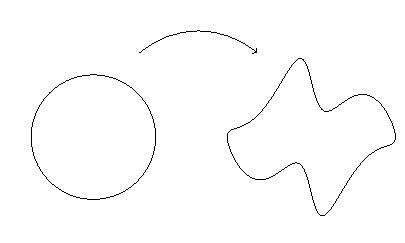
\includegraphics[width=0.9\linewidth]{circle_mapping.pdf}}
  \caption{A simple shape. We can think of a shape as the whole mapping, or simply as the subset to the right.}
\end{figure}

\subsection*{The manifold of parametrized curves -- $\I(\S^1, \R^2)$}
\label{sec:parametrized-curves}

The first structure we want to impose on our manifold of curves is tangent spaces and tangent vector to our elements in the space.

For ordinary finite dimensional manifolds $M$ \hl{we have so far worked with} the definition of tangents vectors as \textit{derivatives}. This is a rather abstract construction, which, however, turns out to be nice to work with. Fortunalety, we know that this definition corresponds to the more geometrically intuitive definition of tangent vectors at a point $m \in M$ as derivatives of paths going through $m$. We shall use this a motivation for our definition of tangent vectors to points in $\I$.

Consider a point $c\in \I$ and a path in $\I$ defined around $0$ that goes through the point $c$. This path is a map
\begin{equation}
  \label{eq:path-in-imm}
  [-\epsilon, \epsilon] \ni t \mapsto  q(t, \blank) :=  (\theta\mapsto q(t, \theta)) \in \I,
  \quad q(0,\theta) = c(\theta),
\end{equation}
i.e., for each $t$ we get a parametrized curve, and at 0 we get the curve $c$. We can also think of this a (smooth) map
\begin{equation*}
  [-\epsilon, \epsilon] \times \S^1  \ni (t, \theta) \mapsto q(t, \theta) \in \R^2.
\end{equation*}
As in the finite dimensional case we can now take the \textit{time derivate} of our path and evaluate this at 0; of course, this is technically not obvious, as our constructed path maps into a function space, but we shall here simply take this derivative to be understood pointwise:

\begin{definition}
  The tangent space $T_{c}\I$ to an element $c \in \I$ consists of all function
  $h\colon \S^1 \rightarrow \R^2$ such that
  \begin{equation*}
    h(\theta) = q_t(0, \theta) := \frac{\partial }{\partial t} \bigg\vert_{t=0} q(t,\theta),
  \end{equation*}
  where $q$ is some path passing through $c$ at 0 (as defined in \eqref{eq:path-in-imm}).
\end{definition}

By this definition, we can essentially think of tangent vectors in $\I$ as vector fields on the circle. Figure~\ref{fig:def-tang-imm} illustrates the idea behind the definition.

\begin{figure}
  \centering
  \begin{subfigure}{.49\textwidth}
    \centering
    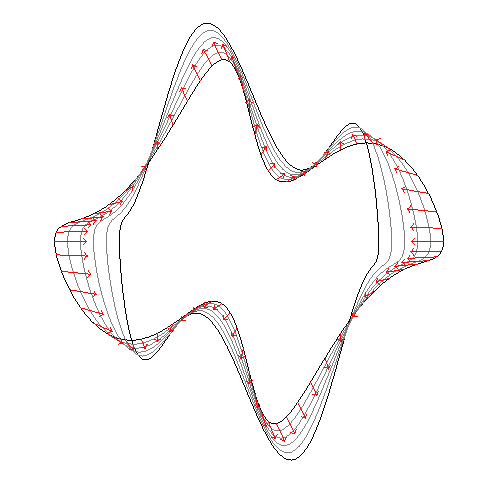
\includegraphics[width=1\linewidth]{path.pdf}
  \end{subfigure}
  \begin{subfigure}{.49\textwidth}
    \centering
    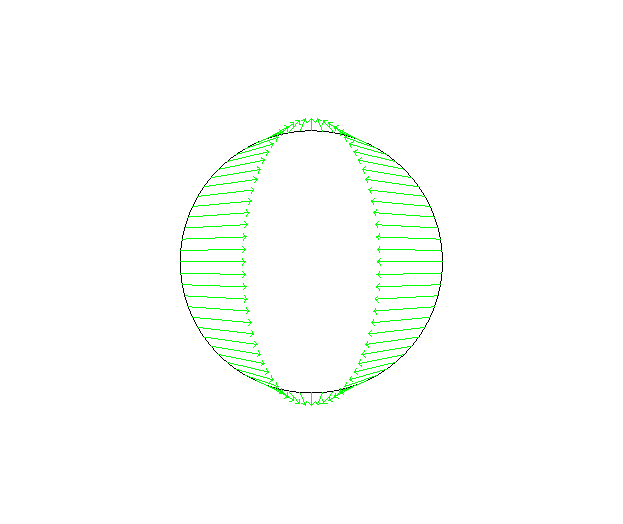
\includegraphics[width=0.8\linewidth]{circle_vectorfield.pdf}
  \end{subfigure}
  \caption{Illustration of tangent vectors in $\I$. The left illustration shows a path in the space of curves and how to obtain a tangent vector from this. The right illustration shows how to think of this tangent vector as a vector field on the circle.}
  \label{fig:def-tang-imm}
\end{figure}

We want to make our space of curves into a Riemmanian manifold so the next step is to impose a metric
\hl{[why do we/others call it a metric -- shouldn't it be an inner product?]}
on the tangent spaces. Because the tangent spaces are function spaces, the most obvious metric to use is some version of the $\mathrm{L}^2$ metric.

\begin{definition}
  The \textit{$\mathrm{G}$ metric} or \textit{$\mathrm{G}_c$ metric} at the point $c \in \I$ is defined as
  \begin{equation*}
    \mathrm{G}_c(h,k) :=
    \left(
      \int_{\S^{1}} \left\langle{h(\theta)
          , k(\theta)}\right\rangle |c_{\theta}| \diff \theta
    \right)^{\frac{1}{2}},
  \end{equation*}
  $h,k \in T_cB = C^{\infty}(\S^1,\R^2)$.
\end{definition}

Adding the parameter derivative $c_{\theta}$ makes the metric invariant to reparametrizations which is essential when we want to let this fall down as a metric on $\mathcal{I}$. From this definition it is straightforward to define a notion of \textit{length} of a path in $\I$ which again allows us to define a \textit{distance} between two point in our space of curves. By defintion, the pointwise time derivative at $t$ of a path $t \mapsto q(t, \blank)$ in $\I$ is a tangent vector to the curve $q(t,\blank)$, so the following definition makes sense.

\begin{definition}
  \label{def:length-in-imm}
  Let $t \mapsto q(t,\blank)$ be a path in $\I$ with $t \in [0,1]$. The \textit{length} of the path $q$ with respect to the $\mathrm{G}$ metric  is
  \begin{equation*}
    L(q) := \int_{0}^{1} \mathrm{G}_{q(t,\blank)}(q_t,q_t) \diff t =
    \int_{0}^{1}
    \left(
      \int_{\S^{1}} \|q_t\|^2 |q_{\theta}| \diff \theta
    \right)^{\frac{1}{2}}
    \diff t.
  \end{equation*}
  The \textit{geodesic distance} \hl{[geodesic?]} between to curves $b,c \in \I$ (with respect to the $\mathrm{G}$ metric) is
  \begin{equation*}
    D(b,c) := \inf_{q \in \mathcal{Q}} L(q),
  \end{equation*}
  where $\mathcal{Q}$ denotes all paths $q$, such that $q(0,\blank)=b$ and $q(1,\blank)=c$.
\end{definition}


\subsection*{The manifold of unparametrized curves -- $\mathcal{I}(\S^1, \R^2)$}
\label{sec:manif-unpar-curv}

Using the setup from the previous section, we now define a manifold structure on $\mathcal{I}$. As it is easiest to represent element of this space with element from $\I$, we are particularly interested in how to calculate the length of a path in $\mathcal{I}$ directly from a parametrized representative of this path in $\I$. For a parametrized curve $c \in \I$ we write $\pi(c) := \mathrm{Im}(c)\in \mathcal{I}$ for the projection onto the quotient space, and we refer to $c\in\I$ as a \textit{(parametrized) representative} for $\pi(c) \in \mathcal{I}$. Similarly for a path $q = q(t, \blank) \in \I$ we construct the projection $\pi(q) = \pi(q(t,\blank)) \in \mathcal{I}$ and refer to $q$ as a representative for $\pi(q)$.

First of all we need to know how the tangent vectors of the quotient space $\mathcal{I}$ look like. We cannot directly use the same approach as in the previous subsection, because our definition of tangent vector would then be
sensitive to reparametrizations: Consider a time-dependent
reparametrization $\phi(t,\theta)$, or, equivalently, a path $t \mapsto \phi(t,
\blank)$ in $\text{Diff}(\S^1)$; then the two paths $t \mapsto
\pi(q(t, \blank))$ and $t \mapsto \pi(q(t, \phi(t, \blank)))$ are
identical in $\mathcal{I}$ but give rise to two different vector fields.

To make better sense of the tangents vectors of the quotient space, we
use the following result.

\begin{proposition}
  \label{prop:horizontal-path}
  For every path $t \mapsto q(t, \blank)$ in $\mathrm{Imm}$ there exists a
  time-dependent reparametrization $t \mapsto \phi(t, \blank) \in
  \mathrm{Diff}(\S^{1})$ such that the path
  \begin{equation*}
    t \mapsto \tilde{q}(t, \theta):=q(t, \phi(t,\theta))
  \end{equation*}
  fulfills
  $\langle \tilde{q}_t, \tilde{q}_{\theta}\rangle=0$ for all $(t,\theta) \in [0,1]\times \S^1$, and such that $\phi(0, \theta)=\theta$. Furthermore, it holds that
  \begin{equation}
    \label{eq:canon-repar}
    \phi_t = a \circ \phi
    = -\frac{\langle q_t \circ \phi, q_{\theta} \circ \phi\rangle}{|q_{\theta}\circ \phi|^2},
    \quad a := -\frac{\langle q_t,
      q_{\theta}\rangle}{|q_{\theta}|^2}.
  \end{equation}
\end{proposition}

\begin{proof}
  \hl{todo or ref.}
\end{proof}

\begin{remark}
  \label{remark:ortho-decom}
  \begin{enumerate}
  \item  When we write $\tilde{q}$ in the following, we shall we refer to a path obtained from another path $q$ by reparametrizing with $\phi$ above.
  \item Note that for every vector field $h \in T_c(\I)$, determined from the path $q$, we can make a pointwise decomposition of $h$ onto $q_{\theta}(0, \blank)$ and $iq_{\theta}(0, \blank)$ by using the pointwise orthogonal projection. Explicitly we have that
  \begin{equation*}
    h = q_t = p_{q_{\theta}}(q_{t}) + p_{iq_{\theta}}(q_{t}),
  \end{equation*}
  where $p$ is taken to be the standard \textit{pointwise} $\R^2$ orthogonal projection, which is given as
  \begin{equation*}
    p_v(u) = \frac{\langle v, u \rangle}{|v|^2} v, \quad u, v \in \R^2.
  \end{equation*}
  More correctly we should thus write
  \begin{equation*}
    h(\theta) = q_t(0,\theta) = p_{q_{\theta}(0,\theta)}(q_{t}(0,\theta)) +
    p_{iq_{\theta}(0,\theta)}(q_{t}(0,\theta)).
  \end{equation*}
  From this we see that the time derivative of the reparametrization in the previous Proposition is the coefficient function for the projection onto the parameter derivative of the original path $q$; this becomes relevant in a moment.
\end{enumerate}
\end{remark}

We can use this result to define tangent vectors to elements of $\mathcal{I}$ in
a consistent way:

\begin{definition}
  \label{def:tang-quotient}
  A \textit{tangent vector} $h$ to an element $\pi(c) \in \mathcal{I}$ is defined as a vector fields obtained from some path $(-\epsilon, \epsilon) \ni t \mapsto q(t, \blank) \in \I$, with $q(0,\blank) = c$, by
  \begin{equation}
    \label{eq:tang-quotient}
    h(\theta) = \frac{\partial }{\partial t} \bigg\vert_{t=0} \tilde{q}(t,\theta)
    = \frac{\partial }{\partial t} \bigg\vert_{t=0} q(t, \phi(t,\theta)),
  \end{equation}
  with $\tilde{q}$ and $\phi$ given in accordance with remark~\ref{remark:ortho-decom}.

  \hl{[NB: Does this actually solve the problem about define the ubiquity in defining tangent vectors? Not clear that applying $\phi$ to a reparametrization of $q$ will yield the same result? However, it shows that we can always think of are path as moving orthonormally; but maybe we should compine this definition with the proposition below?]}
\end{definition}

First we note that this gives us the following visualization of the tangents spaces of $B$.

\begin{proposition}
The tangent space to an element $\pi(c) \in \mathcal{I}$ consists of orthonormal vector fields on the circle, i.e.,
  \begin{equation*}
    T_{\pi(c)}(\mathcal{I}) =
    \left\{
      b i c_{\theta} \mid b \in C^{\infty}(\S^1,\R)
    \right\}.
  \end{equation*}
\end{proposition}

\begin{proof}
  This follows from Definition~\ref{def:tang-quotient} and the property of the reparametrization $\phi$.
\end{proof}

As the length of a path in $\mathcal{I}$ is our primary concern, we skip straight to this without actually defining the inner product on the tangent spaces. The central idea is to mimic Definition~\ref{def:length-in-imm} on the reparametrized path $\tilde{q}$; and though we don't bother to go trough a inner product on the tangent spaces, we note that by this construction the time derivative of the path $\tilde{q}$ is a valid tangent vector in $\mathcal{I}$ at every point $\pi(q(t,\blank))$

\begin{definition}
  The \textit{length} in $\mathcal{I}$ of a path $\mathrm{q}=\pi(q)$ is
  \begin{equation*}
    \mathcal{L}(\mathrm{q})= \mathcal{L}(\pi(q)) := L(\tilde{q}) =
    \int_{0}^{1}
    \left(
      \int_{\S^{1}} \|\tilde{q}_t\|^2 |\tilde{q}_{\theta}| \diff \theta
    \right)^{\frac{1}{2}}
    \diff t,
  \end{equation*}
  with $\tilde{q}(t,\theta)=q(t,\phi(\theta))$ as in remark~\ref{remark:ortho-decom}.
  The \textit{geodesic distance} between to shapes $\mathrm{b}, \mathrm{c} \in \mathcal{I}$ represented by $c,b \in \I$, is
  \begin{equation*}
    \mathcal{D}(\mathrm{b},\mathrm{c}) = \mathcal{D}(\pi(b),\pi(c)) := \inf_{q \in \mathrm{Q}} \mathcal{L}(q),
  \end{equation*}
  where $\mathrm{Q}$ denotes all paths $\mathrm{q}$ in $\mathcal{I}$, such that $\mathrm{q}(0)=\pi(b)$ and $\mathrm{q}(1)=\pi(c)$.
\end{definition}

\begin{proposition}
    $\mathcal{L}$ is well-defined, and for any representative $t \mapsto q(t, \blank) \in \I $ of the path $t \mapsto \tilde{q}(t) \in B$ the length can be calculated as
    \begin{equation}
      \label{eq:length-quotient}
    \mathcal{L}(\tilde{q}) = \int_{0}^{1}
    \left(
      \int_{\S^1}  \frac{\langle q_t, i q_{\theta}\rangle^2}{|q_{\theta}|} \diff \theta
    \right)^{\frac{1}{2}} \diff t.
  \end{equation}
\end{proposition}

\begin{proof}
  For ease of notation, write $q \circ \phi$ to mean $q(t, \phi(t,\theta))$ and so on during this proof.
  First, we shows that \eqref{eq:length-quotient} implies that $\mathcal{L}$ is well-defined; so assume \eqref{eq:length-quotient} holds and let $q(t,\blank)$ and $p(t, \blank)$ be two different representatives for $\tilde{q}(t)$. This means that we must have a reparametrization $\psi(t,\theta)$ such that
  \begin{equation*}
    p(t, \psi(t,\theta)) = q(t, \theta).
  \end{equation*}
  Then
  \begin{equation*}
    p_t = q_t\circ \psi + \psi_t (q_t \circ \psi), \quad
    p_{\theta} = \psi_{\theta}(q_{\theta} \circ \psi),
  \end{equation*}
  so
  \begin{equation*}
    \begin{aligned}
      \left\langle
        p_t, i p_{\theta}
      \right\rangle
     &  =     \left\langle
        q_t \circ \psi + \psi_t (q_{\theta} \circ \psi),
        \psi_{\theta} (iq_{\theta} \circ \psi)
      \right\rangle \\
     & =     \left\langle
        q_t \circ \psi,
        \psi_{\theta} (iq_{\theta} \circ \psi)
      \right\rangle \\
      & = (\langle q_t, i q_{\theta}\rangle \circ\psi) \psi_{\theta},
    \end{aligned}
  \end{equation*}
  and thus
  \begin{equation*}
    \int_{\S^1} \frac{\langle p_t, i p_{\theta}\rangle^2}{|p_{\theta}|} \diff \theta
    =
    \int_{\S^1}
    \left(
      \frac{\langle q_t, i q_{\theta}\rangle^2}{|q_{\theta}|}
    \right) \circ \psi |\psi_{\theta}| \diff \theta
    =    \int_{\S^1}
      \frac{\langle q_t, i q_{\theta}\rangle^2}{|q_{\theta}|}  \diff \theta,
    \end{equation*}
    which shows that the length does not depend on the parametrization of the path.

  Next, by construction, the tangent vectors along the path $\tilde{q}$ in $B$ is given as
  \begin{equation*}
    \frac{\partial }{\partial t}  (q \circ \phi)
    = q_t \circ \phi + \phi_t (q_{\theta} \circ \phi)
  \end{equation*}
  Now, as in remark~\ref{remark:ortho-decom}, decompose $q_t \circ \phi $ by projecting pointwise onto $q_t \circ \phi $ and $i q_t \circ \phi $. Then we get
  \begin{equation*}
    q_t \circ \phi =
    % \frac{\langle q_t \circ \phi, iq_{\theta} \circ \phi \rangle}
    % {|q_{\theta} \circ \phi|^2}(iq_{\theta} \circ \phi) +
    % \frac{\langle q_t \circ \phi, q_{\theta} \circ \phi \rangle}
    % {|q_{\theta} \circ \phi|^2}(q_{\theta} \circ \phi),
    % =
    \left(
      \frac{\langle q_t  , iq_{\theta}   \rangle}
    {|q_{\theta}  |^2}iq_{\theta}
  \right) \circ \phi +
  \left(
    \frac{\langle q_t  , q_{\theta}   \rangle}
    {|q_{\theta}  |^2}q_{\theta}
  \right) \circ \phi,
  \end{equation*}
  and by Proposition~\ref{prop:horizontal-path} we see that the last term cancels with
  $\phi_t(q_{\theta}\circ \phi)$, so
  \begin{equation*}
    \frac{\partial }{\partial t} ( q \circ \phi )=
    % \frac{\langle q_t \circ \phi, iq_{\theta} \circ \phi \rangle}
    % {|q_{\theta} \circ \phi|^2}(iq_{\theta} \circ \phi)
    % =
    \left(
      \frac{\langle q_t  , iq_{\theta}   \rangle}
      {|q_{\theta}  |^2}iq_{\theta}
    \right)
    \circ \phi.
  \end{equation*}
  For any fixed $t \in [0,1]$, the reparametrization $\phi$ is just an ordinary reparametrization of the curve $\theta \mapsto q(t,\theta)$, so by invariance of the metric we have that
  \begin{equation*}
    \begin{aligned}
    & G_{q(t,\phi(t,\blank))}^2
    \left( \frac{\partial }{\partial t} ( q \circ \phi ),
      \frac{\partial }{\partial t} ( q \circ \phi )
  \right) \\
  & \quad=  G_{q(t,\phi(t,\blank))}^2
    \left(
          \left(
      \frac{\langle q_t  , iq_{\theta}   \rangle}
      {|q_{\theta}  |^2}iq_{\theta}
    \right)
    \circ \phi,
        \left(
      \frac{\langle q_t  , iq_{\theta}   \rangle}
      {|q_{\theta}  |^2}iq_{\theta}
    \right)
    \circ \phi
    \right) \\
    & \quad =
    G_{q(t,\blank)}^2
    \left(
      \frac{\langle q_t  , iq_{\theta}   \rangle}
      {|q_{\theta}  |^2}iq_{\theta} ,
      \frac{\langle q_t  , iq_{\theta}   \rangle}
      {|q_{\theta}  |^2}iq_{\theta}
    \right) \\
    & \quad =
    \int_{\S^1}
    \left\|
      \frac{\langle q_t  , iq_{\theta}   \rangle}
      {|q_{\theta}  |^2}iq_{\theta}
    \right\|^2 |q_{\theta}  | \diff \theta \\
    & \quad =
    \int_{\S^1}
      \frac{\langle q_t  , iq_{\theta}   \rangle^2}
      {|q_{\theta}  |}  \diff \theta,
  \end{aligned}
\end{equation*}
from which \eqref{eq:length-quotient} follows immediately by definition.
\end{proof}

\hl{Some concluding text...}

\subsection*{\hl{Comparing this to the formal construction as a Frechet manifold}}
\label{sec:hlcomp-this-form}

\hl{... a lot of references ...}

%%% Local Variables:
%%% mode: latex
%%% TeX-master: "local-masters/local-tangent-space-of-curves"
%%% End:


\section{Metrics on the shape space}
\label{sec:metrics-shape-space}
In the previous sections we defined and deduced some properties of our shape space of interest. We also defined a metric induced by the $L^2$-inner product. In this section we consider this metric and another in more depth.

\subsection{The L2 metric vanishes}
\label{sec:l2-metric-vanishes}

In the previous section we went through some work to construct a measure of length for a path $q$ in the space $\mathcal{I}$. As the tangent spaces were seen to consist of some functions on the circle, it was natural to consider using a version of the L$^2$-metric (a version invariant to reparametrizations). However, as we illustrate in this section, this does not give rise to a usable notation of length, because the geodesic distance following from this metric becomes 0 for every two curves in the space.

It can seem weird to go through so much trouble to define a useless distance. But firstly, the construction illustrates some of the difficulties in defining a reasonable notion on length on $\mathcal{I}$; secondly, and more importantly, the fact that the distance vanishes is a quite surprising result, which depends crucially on the formula for the length of a path given in Proposition~\ref{prop:length-quotient}. This gives us some justification for the somewhat unfruitful work of defining the L$^2$-metric.

The ``proof'' below is mostly heuristic, and we only consider the very simple case of a path transforming the circle into a larger circle, but this captures the main idea.
\begin{theorem}
  \label{theorem:l2-metric-vanishes}
  For all $\mathrm{a},\mathrm{b} \in \mathcal{I}$
  \begin{equation*}
    \mathcal{D}(\mathrm{a},\mathrm{b}) = 0.
  \end{equation*}
\end{theorem}

\begin{proof}[Proof of Theorem~\ref{theorem:l2-metric-vanishes}]

  \begin{figure}
    \centerline{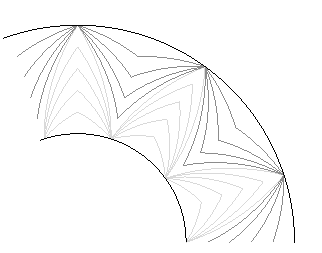
\includegraphics[width=0.6\linewidth]{zigzag-path0.pdf}}
    \caption[]{Illustration of a zigzag path moving the unit circle to the circle with radius 2. The path first moves the points along the path sketched in light-grey and then moves them along the dark-grey path.}
    \label{fig:zigzag-path}
  \end{figure}

  By the definition of the length $\mathcal{D}$ we need to show that for any two paths $\mathrm{a},\mathrm{b} \in \mathcal{I}$ and any $\epsilon >0 $ there exists a path $\mathrm{q}$ in $\mathcal{I}$ such that
  \begin{equation*}
    \mathcal{L}(\mathrm{q}) < \epsilon.
  \end{equation*}
  The trick is to construct a path in $\I$ that moves in zigzag and then use Proposition~\ref{prop:length-quotient} to calculate the length of this path in $\mathcal{I}$.
  It turns out that when we increase the number of teeth of the zigzag path, the length of the path decreases in $\mathcal{I}$.
  The idea of such a zigzag path is illustrated in figure~\ref{fig:zigzag-path}.

  To see why this  phenomenon happens, first rewrite \eqref{eq:length-quotient} from Proposition~\ref{prop:length-quotient} as
  \begin{align*}
    \mathcal{L}(q) &
                     = \int_{0}^{1}
                     \left(
                     \int_{\S^{1}} \frac{\langle q_{t},i q_{\theta}\rangle^2}
                     {|q_{\theta}|}  \diff \theta
                     \right)^{1/2} \diff t \\
                   & =  \int_{0}^{1}
                     \left(
                     \int_{\S^{1}}
                     \left(
                     \frac{\langle q_{t},i
                     q_{\theta}\rangle}{| q_{t}|| q_{\theta}|}
                     \right)^2
                     | q_t|^2   | q_{\theta}|
                     \diff \theta
                     \right)^{1/2} \diff t \\
                   &  =
                     \int_{0}^{1}
                     \left(
                     \int_{\S^{1}}
                     \cos(\alpha( q_t, i q_{\theta}))^2
                     | q_t|^2   | q_{\theta}|
                     \diff \theta
                     \right)^{1/2}\diff t,
  \end{align*}
  with $\alpha(x,y)$ denoting the angle between $x$ and $y$.
  When constructing a zigzag-path the angle will for large enough $n$ be given approximately by
  \begin{equation}
    \label{eq:tan-angle}
    2n \approx \tan(\alpha).
  \end{equation}
  Note that this does not depend on $\theta$ nor $t$.
  See figure~\ref{fig:angle-arg} for a visual justification of this.
  \begin{figure}[h]
    \centering
    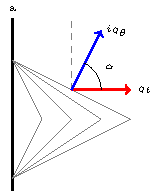
\includegraphics[width=0.5\linewidth]{angle-argument.pdf}
    \caption{Relative to $q_t$, $iq_{\theta}$ is by construction a line with slope $2n$, and thus the angle between these two vectors are found by \eqref{eq:tan-angle}. Note that the starting curve, $\mathrm{a}$, is here represented as a straight line to simplify the calculations; this should be a reasonable approximation when $n$ is large.}
    \label{fig:angle-arg}
  \end{figure}

  We have that
  \begin{equation*}
    \cos(\arctan(2n)) = (1+(2n)^2)^{-1/2}
    = O(n^{-1}),
  \end{equation*}
  so we can write
  \begin{equation}
    \label{eq:approx-L-angle}
    \begin{aligned}
    \mathcal{L}( \mathrm{q} )
    & =
      \int_{0}^{1}
      \left(
      \int_{\S^{1}}
      O(n^{-1})^2
      | q _t|^2   | q _{\theta}|
      \diff \theta
      \right)^{1/2} \diff t \\
    & =
      O(n^{-1})
      \int_{0}^{1}
      \left(
      \int_{\S^{1}}
      | q _t|^2   | q _{\theta}|
      \diff \theta
      \right)^{1/2} \diff t.
    \end{aligned}
  \end{equation}
  To show that our zigzag path has arbitrary small length we thus just need to show that the remaining integral does not grow faster than $n$. Figure~\ref{fig:zigzag-path-angle} illustrates how the angle $\alpha$ increases towards $\pi/2$, making $\cos(\alpha) \rightarrow 0$; at the same time, it is seen how $q_{\theta}$ grows -- not fast enough, however, to kill the $\cos(\alpha)$ term, it turns out.

\begin{figure}
  \centering
  \begin{subfigure}{.49\textwidth}
    \centering
    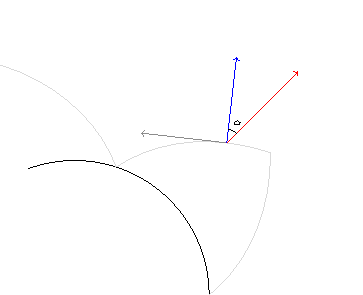
\includegraphics[width=1\linewidth]{zigzag-path.pdf}
  \end{subfigure}
  \begin{subfigure}{.49\textwidth}
    \centering
    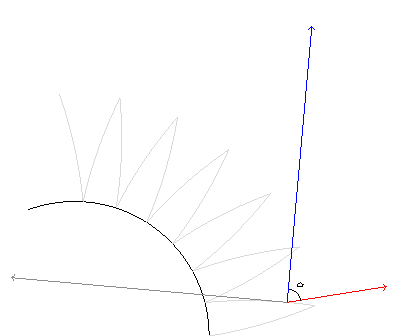
\includegraphics[width=1\linewidth]{zigzag-path2.pdf}
  \end{subfigure}
  \caption{Illustration of how the angle $\alpha$ increases with the number of teeth of the zigzag path. The red vector gives the time derivative, the grey the path derivative, and the blue the normal of the path derivative. The zigzag path is shown in light-grey in the background. (Note that the length of the vectors are scaled to fit the drawing and does not necessarily reflect an exact relationship between the lengths of the two.)}
  \label{fig:zigzag-path-angle}
\end{figure}

As an example, we take the simple case where we expand the circle $e^{i\pi\theta}$ to
$2e^{i\pi\theta}$. The zigzag path is then concretely given as
\begin{equation*}
  \phi(t,\theta) = e^{i\pi\theta}
  \sum_{k=0}^{n-1}
  h^{n,k}(t,\theta) + g^{n,k}(t,\theta)
\end{equation*}
where
\begin{equation*}
  \begin{aligned}
    h^{n,k}(t,\theta) & := 1_{[\frac{k}{n},\frac{k}{n} +
      \frac{1}{2n})}(\theta) \left( 1+2t(n\theta-k) \right), \\
    g^{n,k}(t,\theta) & := 1_{[\frac{k}{n} + \frac{1}{2n},\frac{k+1}{n})}(\theta)
    \left( 1+2t(1-n\theta-k) \right).
  \end{aligned}
\end{equation*}
We have that
\begin{equation*}
  \begin{aligned}
    |\phi_t| & = \sum_{k=0}^{n-1} |h^{n,k}_t| + \sum_{k=0}^{n-1}
    |g^{n,k}_t|, \\
    |\phi_{\theta}| & = \sum_{k=0}^{n-1} |h^{n,k}_{\theta} + h^{n,k} | +
    \sum_{k=0}^{n-1}
    |g^{n,k}_{\theta} + g^{n,k} |,
  \end{aligned}
\end{equation*}
so by symmetry
\begin{equation*}
  \begin{aligned}
    \int_{0}^{1}
    |\phi_t|^2   |\phi_{\theta}|
    \diff \theta
    & =
    2n \int_{0}^{\frac{1}{2n}} |h^{n,0}_t|^2 |h^{n,0}_{\theta} + h^{n,0} |
    \diff \theta \\
    & = 2n \int_{0}^{\frac{1}{2n}}
    (2n\theta)^2(2tn+1+t2n\theta) \diff \theta \\
    & = \int_{0}^1
    u^2(2tn+1+t u) \diff \theta \\
    & = O(n),
  \end{aligned}
\end{equation*}
for $t\in[0,1]$. Plugging this into \eqref{eq:approx-L-angle} gives the result.
\end{proof}

The above result shows that the simple $L^2$-metric is unfortunately not a fruitful way for imposing a metric structure on our shape space. To do this, more complicated metrics that take more of the functions properties into account is needed. One fairly straightforward generalisation of the $L^2$ metric are Sobolev metrics that take some of the derivatives of a function into account. Another approach is to consider so-called \textit{almost local metric}, which we do in the following section.


%%% Local Variables:
%%% mode: latex
%%% TeX-master: "mainfile"
%%% End:

\section{Almost local metrics}
\label{sec:al-metrics}

The problem at hand is the following: we wish to construct a notion of distance between two points in $B_e(S^1,\R^2)$ by defining a metric, such that the distance between two points is the length of geodesics between the points. As we have seen, the distance induced by the $L^2$-metric vanishes on $B_e(S^1, \R^2)$, so we seek to define metrics, which do not vanish. One type of such metrics is $\textit{almost local metrics}$, which, given $f \in B_e(S^1, \R^2)$, are metrics of the form
\begin{align*}
G_f^\Phi (h,k) = \int_{S^1} \Phi(\text{Vol}(f), H_f, K_f) \bar{g}(h,k) \text{vol}(f^* \bar{g}),
\end{align*}
where $\Phi: \; \R^3 \rightarrow \R_{> 0}$ is smooth, $\text{Vol}(f) = \int_{S^1} \text{vol}(f^* \bar{g})$ is the total volume of $f(S^1)$, $H_f$ is the mean curvature of $f$ and $K_f$ is the Gauss curvature of $f$. Both $H_f$ and $K_f$ are local invariant properties with respect to the Riemanninan metric, defined to be the trace and the determinant of the Weingarten mapping, respectively, and so $\Phi$ is often chosen to only depend on one of the two curvatures. In the case of $f \in B_e(S^1, \R^2)$, $H_f(\theta) = \frac{\det(f_\theta, f_{\theta \theta})}{\left| f_\theta \right| ^3}$, which is just the usual formula for curvature of a plane curve.\\[0.2 cm]
$\Phi$ can also be seen as map from Imm$(S^1, \R^2)$ to $C^\infty (S^1, \R_{> 0})$. When viewed as such, in order for the metric to be invariant under reparametrizations, $\Phi$ must also be equivariant with respect to the action of the diffeomorphism group, Diff$(S^1)$ - i.e. $\Phi(f \circ \phi) = \Phi(f) \circ \phi$ for $\phi \in$ Diff$(S^1)$. \\[0.2 cm]
The total volume of $f$, $\text{Vol}(f)$, is defined via the volume form induced by the pullback metric, $f^*\bar{g}$, so this definition of almost-local metrics only applies to manifolds of embeddings from manifolds which posses a volume form. All compact, oriented manifolds do this, such as $S^1$, (\hl{Reference?}), and almost local metrics are often defined for embeddings from this class of manifolds to $\R^n$. In the case of $f \in B_e(S^1, \R^2)$, the volume form on $S^1$ induced by $f$, is given by vol$(f^*\bar{g}) = \left| f_\theta \right| d \theta$. (\hl{Reference to Riemannian Geometries on Spaces of Plane Curves 2.2}). In our case, almost local metrics therefore take on the form
\begin{align*}
G_f^\Phi (h,k) = \int_{S^1} \Phi(\text{Vol}(f), H_f, K_f) \bar{g}(h,k) \left| f_\theta \right| d \theta.
\end{align*}
Vol$(f)$ is a non-local property of $f$, and thus the metrics are not only dependent on the local properties, $K_f, H_f$, but must be $\textit{almost}$ local metrics. \\[0.2 cm]

\begin{remark}
Both curvatures and the volume form of $f \in B_e(S^1,\R^2)$ take on a particular nice form, but expressions can also be found for the general case where $f \in  B_e(M, \R^n)$ with $M$ a compact orientable $n-1$ dimensional manifold. This is done by using the Levi-Civita connections of the Riemannian manifolds $(\R^n,\bar{g})$ and $(M,G^\Phi)$ to construct the Weingarten mapping. See sections $3.4$ and $3.9$ of \hl{Almost local metrics on shape space of hypersurfaces in $n$-space}   
\end{remark}

Note that if $\Phi$ depends only on $f$ through Vol$(f)$ then $G_f^\Phi (h,k)$ is equal to the L$^2$-metric (up to a constant) (\hl{is this obvious from our definition of the L$^2$ metric ?}). But if $\Phi$ actually depends on either curvature and the total volume, then point-separation is achieved under certain conditions imposed on $\Phi$;

\begin{theorem}\label{point_sep}
If $\Phi(\text{Vol} \, (f), H_f, K_f) \geq A H_f$ for some $A > 0$, then $G_f^\Phi$ induces a point-separating metric on $B_e(S^1, \R^2)$.
\end{theorem}


\begin{proof}
The proof is found in section 3 in \hl{Reference til  Riemannian Geometries...} with a specific choice of $\Phi$. We sketch a few ideas of this proof but emphasize that the specific choice of $\Phi$ is not important (\hl{is this actually true? Don't think so. It uses $\Phi \geq 1$. But that is just a scalar condition w.r.t to the $L^2$-metric???}), but merely that $\Phi(f) > AH_f$ for some $A > 0$. \\[0.2 cm]
Given a path of un-parametrized shapes, $\pi(c) \, : \, [0,1] \times S^1 \rightarrow B_e(S^1, \R^2)$, one can choose a path, $c$, in Imm$(S^1, \R^2)$ such that $c(0, \cdot)$ is an immersion of constant speed, $\langle c_t, c_\theta \rangle = 0$ for all $t$ and $\theta$, and $c(t , \theta)$ has constant speed. Let $c$ be such a path, and let
\begin{align*}
\Phi(f) = 1 + A H_f ^2
\end{align*}  
for some constant $A > 0$ (which implies $\Phi(f) \geq AH_f$). Consider the Hilbert space $L^2(S^1, \left| c_\theta(t, \theta) \right| d\theta) = L^2(S^1, \text{vol} (c(t)^* \bar{g}))$. The Cauchy-Schwarz inequality yields
\begin{align*}
\int_{S^1} \left| c_t(t, \theta) \right| \left| c_\theta(t, \theta) \right| d \theta \leq \left(\int_{S^1} \left| c_\theta(t, \theta) \right| d \theta \right) ^{\frac{1}{2}} \left( \int_{S^1} \left| c_t(t, \theta) \right|^2 \left| c_\theta(t, \theta) \right| d \theta   \right) ^{\frac{1}{2}}.
\end{align*} 
The length of the path $c$ is then
\begin{align*}
L_{G^{\Phi}}(c) := \int_0^1  \sqrt{G^{\Phi}_{c(t)}(c_t, c_t)} dt &= \int_0^1 \left( \int (1 + AH_{c(t)}^2 ) \left| c_t(t, \theta) \right|^2 \left| c_\theta(t, \theta) \right| d\theta     \right) ^{\frac{1}{2}} dt \\
& \geq \int_0^1 \left(\int_{S^1} \left| c_\theta(t, \theta) \right| d \theta \right) ^{-\frac{1}{2}} \int_{S^1} \left| c_t(t, \theta) \right| \left| c_\theta(t, \theta) \right| d \theta dt.
\end{align*}
The mean value theorem for integrals then yields that there exists $t_0 \in [0, 1]$ such that
\begin{align*}
L_{G^{\Phi}}(c)\geq  \left(\int_{S^1} \left| c_\theta(t_0, \theta) \right| d \theta \right) ^{-\frac{1}{2}} \int_0^1 \int_{S^1} \left| c_t(t, \theta) \right| \left| c_\theta(t, \theta) \right| d \theta dt,
\end{align*}
where the first factor is the curve length of $c(t_0, \cdot)$ to the power of $-\frac{1}{2}$, and the second factor can be written as
\begin{align*}
\int_0^1 \int_{S^1} \left| c_t(t, \theta) \right| \left| c_\theta(t, \theta) \right| d \theta dt = \int_0^1 \int_{S^1} \left| \det (d c(t, \theta) \right| d \theta dt,
\end{align*}
which is the area in $\R^2$ swept out by the path $c$ (\hl{make a figure}). We note that if the shape is not trivially a point in $\R^2$ (such that the length at time $t_0$ is $0$) and if the path is not trivial (such that $c(0, \cdot) = c(1, \cdot)$), then this lower bound is strictly positive. Thus any path from two distinct shapes have length greater than $0$, such that the metric induces a point-separating distance function. 
\end{proof}


No matter the choice of $\Phi$, an almost local metric is never point-separating on Imm$(S^1, \R^2)$ - the shape space without quotienting out reparametrizations. To see this let $f \in$ Imm$(S^1, \R^2)$ and take $\tilde{f}$ to be in the orbit of $f$ of the Diff$(S^1)$ action - i.e. $\tilde{f} = \phi \circ f$ for some $\phi \in$ Diff$(S^1)$. Since $\Phi$ is equivariant w.r.t. the action of Diff$(S^1)$, 
\begin{align*}
G_{\tilde{f}}^\Phi (h,k) = \int_{S^1} \Phi(\tilde{f}) \bar{g}(h,k) \text{vol}(f^* \bar{g}) = \int_{S^1} \Phi(f) \circ \phi \bar{g}(h,k) \text{vol}(f^* \bar{g}),
\end{align*}
the almost local metric restricted to the orbit of $f$ can be viewed as a weighted $L^2$-type metric with weights represented by $\Phi(f) \circ \phi$. As the geodesic distance function induced by weighted $L^2$ metrics vanishes (\hl{Reference or follows easily from proof?}), the almost local metric vanishes for point in Imm$(S^1, \R^2)$ which are in the same orbit of the Diff$(S^1)$-action.
\\[0.2 cm]
In general, existence and uniqueness of geodesics w.r.t. almost local metrics are not ensured and thus the length of a path in $B_e(S^1,\R^2)$ cannot be determined by constructing a geodesic and computing its length (\hl{Reference to first article page 11}). In certain cases however, the length of a path is exactly the lower bound used in \ref{point_sep} \hl{Reference to theorem 3.1 in H0 type Riemannian metrics on the space of planar curves}.

\begin{example}
Define an almost local metric on $B_e(S^1, \R^2)$ as above with $\Phi(f) = \ell(f)$ where $\ell(f)$ is the ordinary curve length of $f$ (which implicit is a function of the curvatures of $f$). Let $q_0, q_1 \in B_e(S^1, \R^2)$ be shapes and let $c \, : \, [0,1] \rightarrow B_e(S^1, \R^2)$ be a path from $q_0$ to $q_1$ such that $c(0) = q_0$ and $c(1) = q_1$. The length of the path $c$ is then the area swept out by $c$ in $\R^2$,
\begin{align*}
L_{G^\Phi}(c) = \int_{[0,1]} \int_{S^1} \left| \det dc(t, \theta) \right| d\theta dt,
\end{align*}
and the distance between $q_0$ and $q_1$ is then the infimum over all paths in $B_e(S^1, \R^2)$ which start in $q_0$ and end in $q_1$:
\begin{align*}
d_{G^\Phi}(q_0, q_1) = \inf_{c\in\mathcal{C}} \int_{[0,1]} \int_{S^1} \left| \det dc(t, \theta) \right| d\theta dt,
\end{align*}
where $\mathcal{C}$ denotes all paths $c$, such that $c(0) =q_0$ and $c(1) =q_1$. \\[0.2 cm]
\end{example}

\begin{example}
If $\Phi$ is a more general function of the curve length, $\Phi = e^{A \ell (f)}$, for some constant $A > 0$, then the distance between two shapes, $q_0$ and $q_1$, is bounded by
\begin{align*}
\inf_{c\in\mathcal{C}} \sqrt{A e} \int_{[0,1]} \int_{S^1} \left| \det dc(t, \theta) \right| d\theta dt \leq d_{G^\Phi}(q_0, q_1) \leq \inf_{c\in\mathcal{C}} \sqrt{A e} e^{A \ell_{max}(c) / 2} \int_{[0,1]} \int_{S^1} \left| \det dc(t, \theta) \right| d\theta dt,
\end{align*}
where $\ell_{max} (c) = \max_{t \in [0,1]} \ell (c(t, \cdot))$ is the maximum length of any immersion on the path from $q_0$ to $q_1$. In particular, if $q_0 \neq q_1$, such that there exists no trivial path between the two shapes, then the distance is positive, since the area swept out in $\R^2$ by any path is positive. 
\end{example}





\section{Statistical concepts on shape space}
\label{sec:statistical_concepts_on_shape_space}

If we wish to define statistical concepts like mean and variance on our shape space - the manifold of unparametrized curves - we are faced with some challenges. To begin with our manifold fold is infinite-dimensional, and all theory developed so far in this exposition has been on finite-dimensional manifolds. This is an important part of the generalizations of mean and variance, since we can quite easily define a measure on $M$. If a point $x \in M$ can be written in finitely many local coordinates, a measure can be defined via the use of the metric on the induced (finite) basis of $T_x M$. It is not at all obvious how this method of constructing a measure on $M$ generalizes to the infinite-dimensional case.

For example, the prime example of a infinite-dimensional shape space is a function space, e.g., the space of all continuous function. As is well-known, simply constructing a random variable on such a space is non-trivial; a fundamental construction is the Brownian motion, the existence of which relies on a deep result of Kolmogorov. Our space $\I$ is an example of a restriction of a space of continuous functions (to immersions), and the space $\mathcal{I}$ is even more involved. Thus, simply defining the random points to work with on the shape space promises some challenges.

Secondly, all results regarding existence and uniqueness of mean points have relied on either a global assumption or local assumptions on the Riemannian curvature of the manifold. The behaviour of the curvature of our shape space is not at all well understood, especially since the choice of metric is non-trivial to begin with. One might think that the curvature of $\mathcal{I}$ equipped with the $L^2$-metric is the least difficult to examine, but since the distance function induced by this metric is vanishing, the resulting variance, $\sigma^2_X(y)$ would be $0$ for all random variables $X$ and shapes $y$ (if it is even possible to generalize the variance-formulas in section \ref{sec:mean_and_variance} to the infinite dimensional case.). Thus every point would be a mean point of $X$ which is not a very informative statement.

To make the difficulties stand out explicitly, we write our Definition~\ref{sec:mean_and_variance} when naively replacing the finite-dimensional manifold $M$ with our shape space $\I$ and using an almost local metric. Then we have that $y$ is some fixed shape and $X$ is a random shape (still not defined):
\begin{align*}
  \sigma^2_X(y) &  = \int_{\I}
                  \inf_{\stackrel{c \in \mathcal{C}}{c(0,\blank)=y, c(1,\blank)=z}}
                  L_{G^\Phi}(c)p_X(z)
                  \diff z
  % \\
  %               &  = \int_{\I}
  %                 \inf_{\stackrel{c \in \mathcal{C}}{c(0,\blank)=y, c(1,\blank)=z}}
  %                 \int_{\S^1} \Phi(\mathrm{Vol}(c(t,\blank),H_{c(t,\blank)},K_{c(t,\blank)}),
  %                 \overline{g}(c_t,c_t) |c_{\theta}| \diff \theta
  %                 \diff z \\
  .
\end{align*}
First of all it is not clear that this integral over a function space is well-defined.


%%% Local Variables:
%%% mode: latex
%%% TeX-master: "mainfile"
%%% reftex-default-bibliography: ("litteratur.bib")
%%% End:


\bibliography{litteratur.bib}{}

\end{document}
